\newcommand\blfootnote[1]{%
  \begingroup
  \renewcommand\thefootnote{}\footnote{{\tiny #1 }}%
  \addtocounter{footnote}{-1}%
  \endgroup
}

%%%%%%%%%%%%%%%%%%%%%%  TITLE PAGE  %%%%%%%%%%%%%%%%%%%%%%%%%%%%%%%%%%%%%%%%%%%%
%\begin{frame}
%	%%automatiche from prof theme...
%	%\titlepage
%	%Studente: Andrea Di Iorio	Relatore: Salvatore Filippone
%	%manual cover page
%	\begin{center}
%	\par\noindent\rule{\textwidth}{0.4pt}	%\HRule 
%	\vspace{.7cm}
%	{\Large \bfseries Sparse Triple Matrix Matrix Multiplication\\for\\AlgebraicMultiGrid}
%	\vspace{.7cm}
%	\par\noindent\rule{\textwidth}{0.4pt}	%\HRule 
%	\end{center}
%	\vfill \vspace{0.5cm}
%	\begin{minipage}[t]{0.4\textwidth}
%	\begin{flushleft} \large
%	\emph{Relatore: Salvatore Filippone}\\
%	\end{flushleft}
%	\end{minipage}
%	
%	\begin{minipage}[t]{0.4\textwidth}
%	\begin{flushright} \large
%	\emph{Studente:  Andrea Di Iorio\\Matricola: 0277550}\\
%	\end{flushright}
%	\end{minipage}
%\end{frame}

\begin{frame}

\includegraphics[width=\linewidth,keepaspectratio]{titlePageFull_InProgress.svg.pdf}
\end{frame}
%%%%%%%%%%%%%%%%%%%%%%  TITLE PAGE  %%%%%%%%%%%%%%%%%%%%%%%%%%%%%%%%%%%%%%%%%%%%
\begin{frame}	{Outline}
	\tableofcontents
\end{frame}

\section{Introduzione}
\begin{frame}	{Problema Affrontato}
\begin{itemize}
	\item	Progettare e realizzare implementazioni parallele mediante \emph{openMP} \\
			del triplo prodotto tra matrici sparse (\emph{Sp3MM})
	\item	Necessarie nella fase di setup dei metodi Algebraic Multi Grid (\emph{AMG})
	\begin{itemize}
		\item	in combinazione di solutori iterativi di sistemi di sistemi lineari sparsi \\$Ax=b$
		\item	Prodotto di Galerkin:\\
			$A_{l+1} = (P_l)^T \cdot A_l \cdot P_l  \quad \text{dove:} 
			\begin{aligned}  
				& A \in \mathbb{R}^{n \times n} \\  
				& A_0 = A\\  
				& A_{l+1}  \in \mathbb{R}^{n_{l+1} \times n_{l+1}} \quad \text{con}~ n_{l+1}<n \end{aligned} $%\right\}$%~l=0,\dots,nl-1
	\end{itemize}

\end{itemize}
\centering
\includegraphics[width=.33\linewidth,keepaspectratio]{Multigrid_Visualization_wikipedia.png}
\end{frame}

\section{Algoritmi Esistenti}
\begin{frame} {Formulazioni SpMM}
Considerando la moltiplicazione tra matrici sparse $C = A\cdot B$
\voidLine
\centering
$
\begin{aligned}
  &\text{Row-by-row}	&& \qquad c_{i*} = \sum\limits_{k \in I_i(A)}  a_{ik} \ast  b_{k*}  \\
  &\text{Col-by-col}	&& \qquad c_{*j} = \sum\limits_{k \in I^j(B)}  a_{*k} \ast  b_{kj}   \\
  &\text{Inner-product}	&& \qquad c_{ij} = \sum\limits_{k \in I_i(A) \cap I^j(B) }  a_{ik} \ast  b_{kj}   \\
  &\text{Outer-product}	&& \qquad C = \sum\limits_{i=1}^k  a_{*i} \otimes  b_{i*}                \\
\end{aligned}
$\\
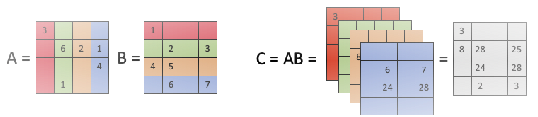
\includegraphics[width=.33\linewidth,keepaspectratio]{outerProductExampleVisual_ESC.png}

\blfootnote{Gao, Jianhua \& Ji, Weixing \& Tan, Zhaonian \& Zhao, Yueyan
«A Systematic Survey of General Sparse Matrix-Matrix Multiplication»}
%Notazione:
%I_I: indici di rigai, I^j indici di colonna j, I(i,j): indici di elementi non zero riga e col
%Outer product: somma di matrici a rango 1 generate dal Prodotto diadico
\end{frame}

\begin{frame} {Algoritmo di Gustavson}
\begin{columns}
	\column{0.65\textwidth}
	\includegraphics[width=.87\linewidth,keepaspectratio]{gustavsonRigheSysSurvey_noLabel.svg.pdf}
	
	\column{0.35\textwidth}
  	Formulazione row-by-row $c_{i*} = \sum\limits_{k \in I_i(A)}  a_{ik} \ast  b_{k*}$
	\voidLine
	\voidLine
	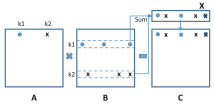
\includegraphics[width=.87\linewidth,keepaspectratio]{gustavsonRigheGraphicalIntel.svg.pdf}
	
\end{columns}
\blfootnote{Fred G. Gustavson «Two Fast Algorithms for Sparse Matrices: Multiplication and Permuted Transposition» 1978}
%Ri-adattamento estremamente compatto pseudocodice di algo gustvson SERIALE (3.4), originariamente basato su un accumulatore denso, 
%switch array per evitare acc. resets
%Paper molto citato, tra I primi contributi nell'ambito della moltiplicazione tra matrici SPARSE

\end{frame}

\begin{frame} {Formulazioni multi dimensionali}
\begin{columns}
	\column{0.70\textwidth}
	\begin{itemize}
		\item	ogni moltiplicazione di elementi non zero $a_{ik} \ast b_{kj}$\\
				(min. operazione assegnabile) è rappresentabile con voxel W(i,j,k)
		\item	sottoinsiemi di W ottenuti fissando uno o due indici
		\begin{itemize}
			\item	Layers: W(i,:,:),W(:,j,:),W(:,:,k)
			\begin{itemize}
				\item	Partizionamento 1D
			\end{itemize}
		\end{itemize}
		\begin{itemize}
			\item	Fibers: Intersezioni di Layers relativi a indici diversi, e.g. W(i,j,:)
			\begin{itemize}
				\item	Partizionamento 2D
			\end{itemize}
		\end{itemize}
		\begin{itemize}
			\item	Cuboid: Sottoinsiemi di W 	
			\begin{itemize}
				\item	Partizionamento 3D
			\end{itemize}
		\end{itemize}
	\end{itemize}
	\column{0.30\textwidth}
	\includegraphics[width=.87\linewidth,keepaspectratio]{MM_cube.svg.pdf}
	\voidLine
	\voidLine
	\voidLine
	\includegraphics[width=.87\linewidth,keepaspectratio]{workCube3D.svg.pdf}
		
\end{columns}

%(Vari paper citano) Rappresentazione op: SpMM in un cubo di lavoro W , faccie A,B->C
%suddivisione lavoro in partizioni cubo
\end{frame}

\begin{frame} {Partitioned SpGEMM}
\begin{columns}
	\column{0.70\textwidth}
	\begin{itemize}
		\item	Partizionamento 2D del calcolo di C
		\begin{itemize}
			\item	Blocchi di C associati a gruppi di righe di A e colonne di B
		\end{itemize}
		\item	Tradeoff tra:
		\begin{itemize}
			\item	overhead associato al partizionamento B 
			\item	Beneficio: |accumulatore denso| < |cache L2|
		\end{itemize}
	\end{itemize}
	\column{0.30\textwidth}
	\includegraphics[width=.87\linewidth,keepaspectratio]{gustavsonRigheBlocksGraphicalIntel.svg.pdf}
\end{columns}
%Sulla quale mi sono un pò più ispirato, ottimi risultati misurati rispetto a varie lib di alg.sparsa disponibili tra cui intel MKL
%BENEFICIO: accDenso fittato in cache(L2) -> durante le accumulazioni evito di andare a richiamare (CONTINUAMENTE) reg. Di memoria da strati cache inferiori (LLC/RAM)
%Overhead B: partizionamento in CSR separate + hyperSparsità => overhead di mem bandwidth … non molto chiaro
%Euristica sul vantaggio d'uso partizi
%e\_nnz = \frac{\sum\limits_{i:e\_nnz(i) > L2\_FP\_WORDS} e\_nnz(i)}
%{\sum\limits_{i=1}^m e\_nnz(i)} ~>~0.3
\end{frame}

\section{Fase simbolica:\\Determinazione dimensione del risultato}

\begin{frame}[fragile] {Fase simbolica di SpMM}
\begin{itemize}
	\item	Determinazione della dimensione (di porzioni) del prodotto
	\item	Necessaria per evitare allocazioni dinamiche durante l'esecuzione parallela
	\begin{itemize}
		\item	e.g. non in linea con la filosofia OpenMP (e.g. \verb|#pragma omp cancel| default off)
	\end{itemize}
	\voidLine
	\voidLine
	\item	UpperBound nel caso row-by-row (formulazione $c_{i*} = \sum\limits_{k \in I_i(A)}  a_{ik} \ast  b_{k*}$):\\
	$| I_i(C) |~\leq~\sum\limits_{ j \in I_i(A) }  | I_j(B)  |$
	\begin{itemize}
		\item	Basso costo computazionale
		\item	Necessità di salvare i risultati intermedi in uno spazio temporaneo
	\end{itemize}
	\item	Calcolo accurato
	\begin{itemize}
		\item	Determinazione esatta 
		\item	Salvataggio degl'indici degli elementi non zero di C
				senza eseguire le operazioni floating-point
		\item	Maggior costo computazionale
		\item	Possibilità di scrivere i risultati intermedi direttamente nella matrice risultante
	\end{itemize}
\end{itemize}
%Focus su necessità di dare ad ogni thread conoscenza dove scrivere il blocco di risultati assegnato CONCORRENTEMENTE
\end{frame}

\begin{frame}[fragile] {UpperBound: Gestione dello spazio temporaneo}
\begin{itemize}
	\item	pre-partizionamento
	\item	Assegnazione dinamica
	\begin{itemize}
		\item	
		\begin{lstlisting}
sparsifyStartV = *@\bfseries \_\_atomic\_fetch\_add@*((acc->lastAssigned),nnz,__ATOMIC_ACQ_REL)
		\end{lstlisting}
		%alternativa con Verbatim
		%\begin{Verbatim}[commandchars=\\\{\}]
		%sparsifyStartV = \verbBoldize{__atomic_fetch_add}((acc->lastAssigned),nnz,__ATOMIC_ACQ_REL)
		%\end{Verbatim}
		\item	
		\begin{lstlisting}
*@\bfseries \#pragma omp atomic capture@*
{ 
sparsifyStartV = acc->lastAssigned;
acc->lastAssigned += nnz;
}
		\end{lstlisting}
		\item In entrambi i casi viene usata:   \verb|lock xadd|
	\end{itemize}
\end{itemize}
%Pre-partizionamento può richiedere formulazione UB ad hoc:
%caso 2D limitare formula precedente a partizioni di colonne... caso triplo prodotto diretto può essere più complicato
%a livello di cache consistency nessun problema grande -> zone di memoria soggette a cacheLines intersecate vengono accedute probabilmente in ordine diverso dai threads...
%
%dynAssign: NO LOCK (omp critical) --> NO FENCE 
%RMW -> atomicamente incremento indice ultimo elem.assegnato ritornando val precedente all'op
%                    (no risultati intermedi visibili tra I thread)
%:::APPROCCI EQUIVALENTI:::
%Lock prefix: consente al processore corrente di avere uso esclusivo di ogni memoria condivisa
%XADD tra nnz,lastIdx -> sparsifyStartV
%
%    accSparseStartIdx = __atomic_fetch_add(&(acc->lastAssigned),nnz,__ATOMIC_SEQ_CST); 
%    3ad2:       48 8b 45 e8             mov    -0x18(%rbp),%rax
%    3ad6:       48 83 c0 18             add    $0x18,%rax
%    3ada:       8b 55 f8                mov    -0x8(%rbp),%edx
%    3add:       f0 0f c1 10             lock xadd %edx,(%rax)
%    3ae1:       89 55 f4                mov    %edx,-0xc(%rbp)
\end{frame}

\begin{frame} {Determinazione accurata}
Percorrendo le operazioni effettuate nella formulazione row-by-row	
($c_{i*} = \sum\limits_{k \in I_i(A)}  a_{ik} \ast  b_{k*}$)
\begin{itemize}
	\item	Si inseriscono gli indici relativi della matrice B 
	come chiavi in una struttura indicizzata
	\item	Porting in Userspace dei RedBlack Tree linux dal kernel 5.10.85 (LTS)
	\item	Uso di un array di bitmaps
	\begin{itemize}
		\item	associando ad ogni indice uno specifico bit
		\item	Analogia con limb di una variabile a precisione arbitraria in GMP
	\end{itemize}
\end{itemize}
%Bitmaps implementati come array di flag generico (uchar array)  ---> similmente in paper originale gustavson
%O array di bitmaps
\end{frame}

\begin{frame}[fragile] {Generazioni di versioni multiple di una funzione a tempo di pre-processamento}
Obiettivi:
\begin{itemize}
	\item	Supportare efficientemente una doppia indicizzazione 
	per l'integrazione in progetto fortran come 
	\url{https://psctoolkit.github.io/products/amg4psblas/}
	\item	Generazione efficiente di varie versioni del prodotto simbolico accurato per implementazioni
	\begin{itemize}
		\item	1D, 2D o triplo prodotto diretto
	\end{itemize}
\end{itemize}
\voidLine
Meccanismo:
\begin{itemize}
	\item	Inclusione multiple dei sorgenti (generici)
	\item	Ri-definizione di macro di configurazione usate nelle funzioni
	\item	Modifica segnatura funzioni derivate mediante pre-processore
\end{itemize}
\voidLine
\begin{lstlisting}
spmat* CAT( spmmRowByRow_SymbNum_ , OFF_F )  ( spmat * A , spmat * B , CONFIG * cfg ){...} 
\end{lstlisting}

%Caso integrazione Fortran (processo di integrazione avviato) molto utile per evitare shifting iniziale complessivo, usato largamente nel codice 
%Multi versioning in generale ( 8 VERSIONI DELLE FUNZIONI BASE):
%Evito uso massiccio di condizioni nel codice (cmq gestiti benissimo da predittori) 
%Esclusione blocchi di codice non necessari 
%  --> maggiore ottimizzabilità in compilazione 
%Segnature diverse da CAT: operatore pre-processore ## wrappato (concat preprocessor token ESPANSI) 
\end{frame}

\section{Fase numerica: calcolo del prodotto tra matrici}
\begin{frame}[fragile]  {Implementazioni multi dimensionali}
\begin{columns}
	\column{0.68\textwidth}
	\begin{itemize}
		\item	Adattamento chunksize per schedule dynamic
		\item	Assegnamento ai thread di blocchi di righe e colonne
		\item	Moltiplicazioni scalari tra
		\begin{itemize}
			\item	$A_{ij}$
			\item	(porzioni) di righe $b_{j*}$
		\end{itemize}
		\item	"Sparsificazione" accumulatore denso
	\end{itemize}

	\column{0.32\textwidth}
	\begin{lstlisting}
((CHUNKS_DISTR_INTERF) cfg->chunkDistrbFunc) (gridSize,AB,cfg);
#pragma omp parallel for schedule(runtime) private(accV,...)
for (tileID = 0; tileID < gridSize; tileID++){
    t_i = tileID/cfg->gridCols;  //i-th row block
    t_j = tileID%cfg->gridCols;  //j-th col block
    colPart = colPartsB + t_j;
    accV = accVectors + tileID; 
    for (ulong r=startRow;  r<startRow+rowBlock;  r++){
        //row-by-row restricted to colsubset of B to get AB[r][:colBlock:]
        for (ulong j=A->IRP[r]-OFF_F,c,bRowStart,bRowLen; j<A->IRP[r+1]-OFF_F; j++){
            //get start of B[A->JA[j]][:colBlock:]
            c = A->JA[j]-OFF_F; // column of nnz entry in A[r][:] <-> target B row
            bRowStart = colPart->IRP[c];
            bRowLen   = colPart->RL[c];
            CAT(scSparseVectMulPart_,OFF_F)(A->AS[j],colPart->AS+bRowStart,colPart->JA+bRowStart,
                bRowLen,startCol,accV);
        }
        accRowPart = outAccumul->accs + IDX2D(r,t_j,cfg->gridCols);
		#if SPARSIFY_PRE_PARTITIONING == T
		_sparsifyUB(accV,accRowPart,startCol);
		#else
        sparsifyUBNoPartsBounds(outAccumul,accV,accRowPart,startCol);
		#endif
        _resetAccVect(accV);
    }
}
if (mergeRowsPartitions(outAccumul->accs,AB,cfg))  goto _err;
	\end{lstlisting}
\end{columns}
\end{frame}	

\begin{frame}[fragile]  {Triplo prodotto Diretto}
\begin{columns}
	\column{0.68\textwidth}
	Calcolo $AC_{i+1} = R \cdot AC \cdot P$
	\begin{itemize}
		\item	Calcolata una riga di $R \cdot AC$ in accumulatore denso
		\item	"Forwardata" immediatamente per indicizzare P
		secondo la formulazione row-by-row
		\item	"Sparsificazione" accumulatore denso $R\cdot AC\cdot P
		Nessuna matrice intermedia prodotta
	\end{itemize}
\column{0.32\textwidth}
	\begin{lstlisting}
#pragma omp parallel for schedule(runtime) private(accRAC,accRACP,c)
for (ulong r=0;  r<R->M; r++){    //row-by-row formulation
    //iterate over nz entry index c inside current row r
    accRAC  = accVectorsR_AC  + omp_get_thread_num();
    accRACP = accVectorsRAC_P + omp_get_thread_num();
	//computing (tmp) R*AC r-th row
    for (idx_t j=R->IRP[r]-OFF_F; j<R->IRP[r+1]-OFF_F; j++)
        CAT(scSparseRowMul_,OFF_F)(R->AS[j], AC, R->JA[j]-OFF_F, accRAC);
    //forward the computed row
    for (idx_t j=0; j<accRAC->nnzIdxMap.len; j++){
        c = accRAC->nnzIdx[j];    
        CAT(scSparseRowMul_,OFF_F)(accRAC->v[c],P,c,accRACP);
    }
    sparsifyUBNoPartsBounds(outAccumul,accRACP,outAccumul->accs+r,0);
    _resetAccVect(accRAC);
    _resetAccVect(accRACP);
}
if (mergeRows(outAccumul->accs,out))    goto _err;
	\end{lstlisting}
\end{columns}
\end{frame}

\section{Performance}
\begin{frame} {Classi di input utilizzati}
\begin{columns}
	\column{0.65\textwidth}
	Ambiente di test
	\begin{itemize}
		\item	OS: CentOS Stream 8
		\item	CPU: Intel Xeon Silver 4210 2.20 GHz 40 core
		\item	RAM: 64GB
	\end{itemize}
	\voidLine
	sistema lineare ottenuto da 
	\begin{itemize}
		\item	discretizzazione alle differenze finite PDE di secondo ordine
		griglia regolare e condizioni al contorno di Dirichlet
		\item	generazione degli aggregati nei AMG
		\begin{itemize}
			\item	Matching
			\item	Vanek-Brezina
		\end{itemize}
		\item	Con e senza Smoothing
		\item	Considerati valori medi di 40 ripetizioni
	\end{itemize}
	\column{0.35\textwidth}
	Matching\\
	\includegraphics[width=\linewidth,keepaspectratio]{sparseMatrices/matchingMediumSmoothed_UnSmoothed.ppm.png}
	Vanek-Brezina\\
	\includegraphics[width=\linewidth,keepaspectratio]{sparseMatrices/varnekBrenzina_MediumSmoothed_UnSmoothed.ppm.png}
\end{columns}
\end{frame}

\begin{frame} {Configurazione}
{\bf Griglia di partizionamento}	\quad strutturazione iterazioni
\begin{itemize}
	\item Implementazioni 1D
	\begin{itemize}
		\item Suddivisione righe in nthread o k*nthread blocchi
	\end{itemize}
	\item Implementazioni 2D
	\begin{itemize}
		\item Suddivisione calcolo di C in blocchi 2D
		da una griglia gridRows X gridCols
		\item Porting \verb|MPI_Dims_create| da OpenMPI
		\begin{itemize}
			\item suddividendo nthread+1 per numeri primi
		\end{itemize}
	\end{itemize}
\end{itemize}
\voidLine
{\bf Schedule Dynamic OpenMP}	\quad assegnamento iterazioni
\begin{itemize}
	\item	Suddivisione it iterazioni in: it/4 chunk (blocchi)
\end{itemize}
\end{frame}

\begin{frame} {Migliore assegnamento spazio temporaneo}
	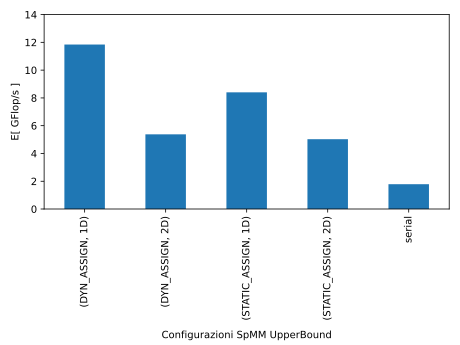
\includegraphics[width=.87\linewidth,keepaspectratio]{graphs/q1.svg.pdf}
\end{frame}
\begin{frame} {Migliore dimensione di bitmap}
	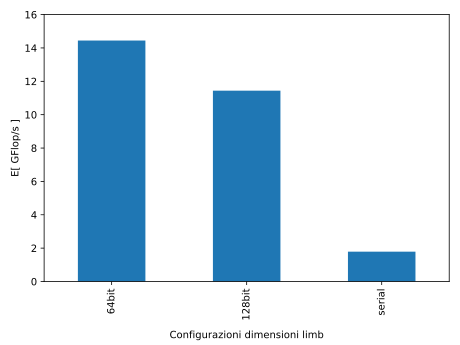
\includegraphics[width=.87\linewidth,keepaspectratio]{graphs/q2.svg.pdf}
\end{frame}

\begin{frame} {Migliore implementazione per classe di input}
\begin{columns}
	\column{.38\textwidth}
	Implementazione/configurazione migliore
	variabile in base alla classe di input
	
	\begin{itemize}
		\item	Triplo prodotto va tendenzialmente meglio
		\item	Maggiore efficienza implementazioni
		su classi di input smoothed
		\item	UpperBound: 1D migliore di 2D 
		in classi Smoothed, 
		\item	viceversa per le classi Unsmoothed
	\end{itemize}
	
	\column{.62\textwidth}
	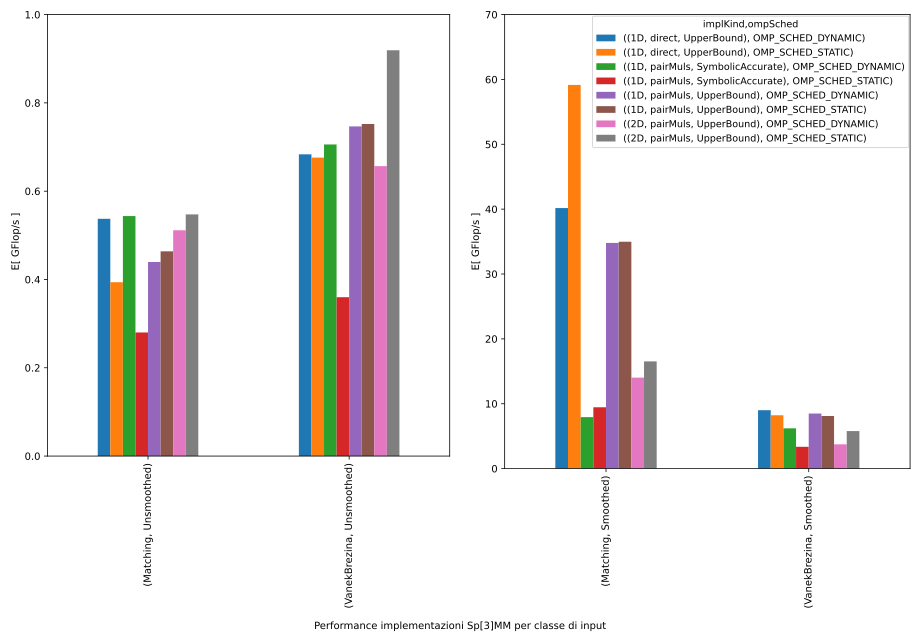
\includegraphics[width=.87\linewidth,keepaspectratio]{graphs/q3.svg.pdf}
\end{columns}
\end{frame}

\begin{frame} {Confronto con implementazione seriale}
\begin{columns}
	\column{.5\textwidth}
	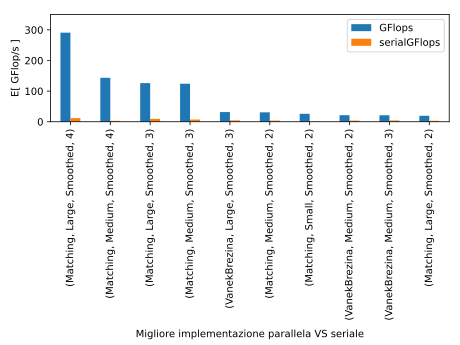
\includegraphics[width=.87\linewidth,keepaspectratio]{graphs/q4-b.svg.pdf}
	\column{.5\textwidth}
	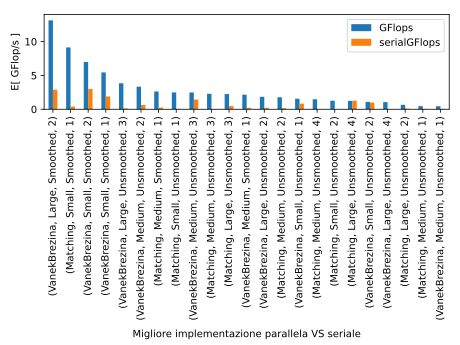
\includegraphics[width=.87\linewidth,keepaspectratio]{graphs/q4-s.svg.pdf}
\end{columns}
\end{frame}
\begin{frame} {Numero thread variabile}
	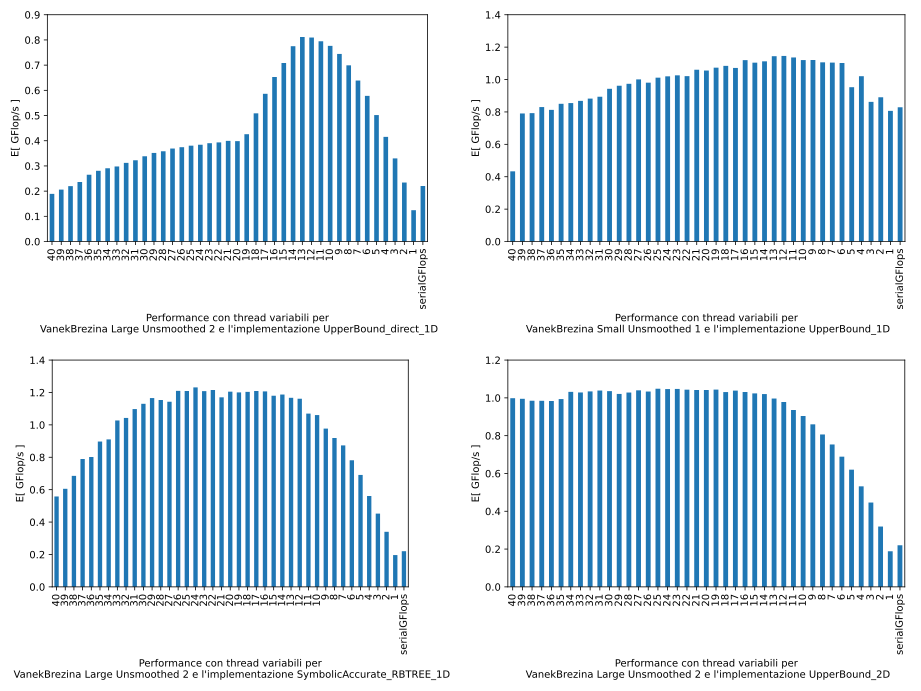
\includegraphics[width=.87\linewidth,keepaspectratio]{graphs/q5.svg.pdf}
\end{frame}
\begin{frame} {Conclusioni}
\begin{itemize}
	\item	Pattern di sparsità dei non zeri degli input 
	determina uno sbilanciamento nel carico di lavoro assegnato
	dipendente da:
	\begin{itemize}
		\item	L'approccio di divisione del lavoro usato
		\item	Tipologia di implementazione
		\item	Livello di concorrenza
	\end{itemize}
	\item	Lo scheduling di un alto numero di thread può essere sconveniente
	\begin{itemize}
		\item	Overhead init/scheduling openMP visibile in config. mono thread
	\end{itemize}
\end{itemize}
\voidLine
Sviluppi futuri
\begin{itemize}
	\item	Analisi dettagliata sul livello di parallelismo ottimale per classe di input
	\item	Estensione implementazioni
	\item	Implementazione formulazioni ESC Outer-Product
\end{frame}
